\chapter{Phase Diversity Experiment} 

\label{PDExp}

%----------------------------------------------------------------------------------------
%	SECTION 1
%----------------------------------------------------------------------------------------

\section{Theoretical Background}



%----------------------------------------------------------------------------------------
%	SECTION 2
%----------------------------------------------------------------------------------------

\section{Experimental Setup}

The design of the experiment was already done by \citet{Bouxin_PDM}.  The setup is built according to her plans and specificationsS.

The experiment is mounted on a pressurized legs optical table. The setup contains six components : a light source, an entrance pupil, an imaging system, a converging lens to focus the beam on the camera, a camera and a wavefront sensor.

\subsection{Light source}

\begin{wrapfigure}{r}{0.4\textwidth}
\centering
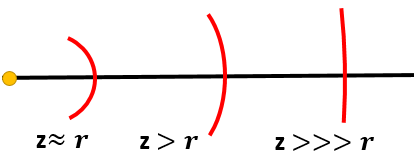
\includegraphics[width=0.4\textwidth]{Figures/WFdistantSource.PNG}
\decoRulewrapFig
\caption[Wavefront curvature]{Wavefront curvature for different source's distances, z. r represents the characteristic size of the arc of interest.}
\label{fig:WFdistantSource}
\end{wrapfigure}

The final application of the phase diversity will be to characterize the optical aberrations induced by the imperfect optical path to a scientific detector of a telescope. For this reason, the light source has to simulate a distant star aberration-free wavefront. A distant star wavefront is considered planar since the object distance, z, is far greater than the telescope size, r, see Fig. \ref{fig:WFdistantSource}. The source of our experiment must then be characterized by planar wavefront.

In order to obtain such a planar wavefront at the entrance pupil, the light source consist of a "pigtailed laser diode", a f=11mm converging lens, a pinhole and a f=200mm converging lens. The pigtailed laser diode, LPS-635-FC \citet{pigtailedLaserDiode}, emits a Gaussian beam centred at 637.5 nm slightly diverging. The converging lens concentrates the beam at the center of the 10$\mu$m pinhole to filter the noise. The second converging lens collimates the beam, obtaining a collimated beam with a planar wavefront.

\begin{figure}
\centering
    \begin{subfigure}{0.5\textwidth}
        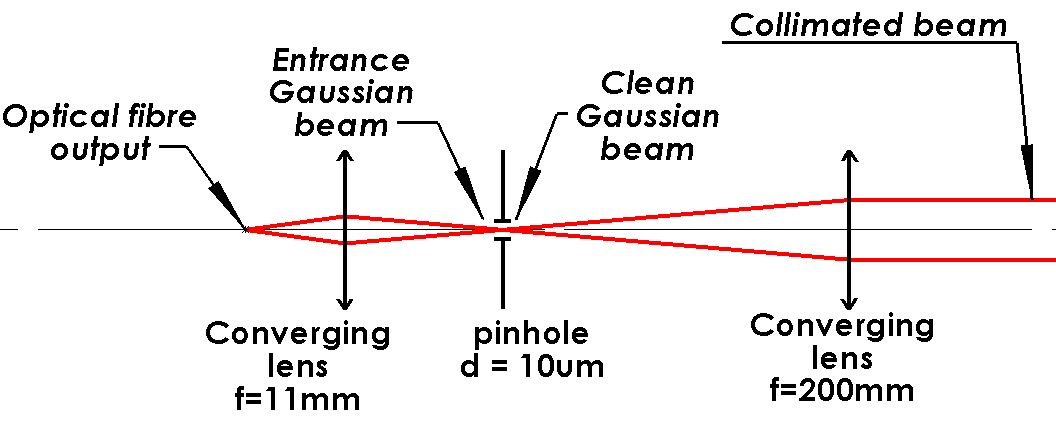
\includegraphics[width=\textwidth]{Figures/source.png}
        \caption{Source ray tracing.}
        \label{fig:sourceRayTracing}
    \end{subfigure}
    \quad
    \begin{subfigure}{0.3\textwidth}
        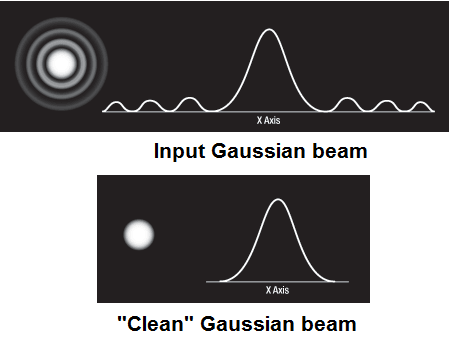
\includegraphics[width=\textwidth]{Figures/pinholeEffect.png}
        \caption{Beam view before and after the pinhole.}
        \label{fig:pinholeEffect}
    \end{subfigure}
    \caption{Source schema and pinhole effect on the beam.}
\end{figure}

\subsection{Entrance pupil}

The entrance pupil of our optical system is a circular aperture of 3.2mm diameter placed after the collimating lens of the light source. 

%------------------------------------------------------------------------------
%	SECTION 3
%----------------------------------------------------------------------------

\section{Results}

This section presents the results of the phase diversity experiment, with the introduction of different sources of aberration.

\subsection{Astigmatism}

The first aberration studied in this work is the astigmatism aberration introduced by a tilted parallel plane plate (link to section). A parallel plane plate introduces astigmatism in addition to the defocus introduced by a plate perpendicular to the optical axis. The astigmatism is due to the fact that symmetric rays with respect to the optical axis have an optical path difference. 
